\chapter{Numerical Assessment}\label{cha:numerical_assesment}
The previous chapter has introduced the FETI method as an efficient implementation of the domain decomposition approach for the purpose of parallelization. However, as any DD method, FETI struggles with some conditioning problems, especially as the number of sub-domains increases.\\
Chapter \ref{cha:feti_solvers} introduced several variations of the original FETI-method. Some of which were derived exactly for the purpose of handling the numerical difficulties. Since all mentioned methods have been implemented into the FEMAC code\cite{FEMAC}, the following chapter provides a profound numerical analysis of the presented methods and their capabilities to handle the heterogeneities along and across the interface, different partitioning schemes, irregular interfaces, incompressibility and inclusion problems. Taking into account the computational effort and scalability issues, conclusions will be drawn, and recommendations will be provided in Chapter~\ref{cha:summary}.
\\
\section{Default parameters}\label{sec:default_parameters}
The previous chapter have already introduced numerous parameters and choices to be made for the FETI solvers. If not explicitly specified otherwise, the following parameters have been used for all calculations in this thesis.
\\
\begin{center}
  \begin{tabular}{|l|l|}
    \hline
    \textbf{Termination criterion} &Residual of $10^{-6}$ \\
    \hline
    \textbf{Preconditioner type}   & Lumped                                               \\
    \hline
    \textbf{A-matrix}              & Unity matrix                                         \\
    \hline
    \textbf{Scaling}               & Multiplicity scaling                                 + K-scaling \\
    \hline
    \textbf{$\rho$ for FETI-AS}    & $0.999$                                               \\
    \hline
    \textbf{FETI-2 coarse grid}    & Geneo with 6 lowest eigenmodes per substructure                            \\
    \hline
  \end{tabular}
\end{center}


\section{Conditioning}\label{sec:condnum}

As explained in Chapter~\ref{cha:introduction}, the FETI type of solvers are hybrids between direct and iterative solvers. A large problem is typically divided into a number of substructures large enough such that each sub-problem can be solved for directly in reasonable time. The hybridization is introduced in the formulation when it comes to solving the connecting interface problem. As explained in Section~\ref{sec:iterative_theory} and outlined algorithmically in Section~\ref{sec:cg}, iterative methods like the Conjugate Gradient algorithm are typically used for this purpose.\\
As any iterative method, a CG algorithm is quite susceptible to bad condition numbers. It should be noted at this point, that the conditioning is a property of the problem formulation, not the algorithm itself. Of course, the absolute value of $\condnum$ depends on the norm used, it should therefore be used only for relative statements.\\

\subsection{Theory}
We consider a linear system of equations
\begin{align}
  \dmat{A} \dvec{x} = \dvec{b} 
\end{align}
We know, that if $det(\dmat{A})=0$, in other words A is singular, this system does not have a solution.\\
If, on the other hand, $det(\dmat{A})\neq 0$, the convergence of an iterative scheme is determined by the condition number defined as $\condnum=\norm{\dmat{A}} \norm{\inv{\dmat{A}}} $.\\
Every iterative algorithm basically works by creating an update on the current solution by considering the residual defined as
\begin{align}
  \dvec{r}^{k}=\dvec{b}-\dmat{A} \dvec{x}^{k} 
\end{align}
The accuracy of the solution is usually defined in terms of the residual as
\begin{align}
  \epsilon=\norm{\dvec{r}}=\norm{\dvec{b}-\dmat{A} \dvec{x}^{k}} 
\end{align}
\\
It his well known that the error will decrease at minimum by a factor of $2 \left( \frac{\sqrt{\condnum}-1}{\sqrt{\condnum}+1} \right)^{i}$ in $k$ steps.


\subsection{Conditioning of the FETI problem}

The previous section indicated, that the condition number of the linear system solved plays a crucial role for the convergence properties of the FETI solver. In fact, some variations like the FETI-Geneo approach explicitly exploit that knowledge by removing "bad components" from the iteration space with the goal of improving the condition number. This chapter will introduce several vivid problem setups that lead to badly conditioned operators. One major challenge are heterogeneities of the material properties along, or across the interface.\\
From an engineering point of view, challenges tend to arise, when the behaviour of a substructure on its own, differs strongly from its behaviour when embedded into the whole system.\\
Figure~\ref{fig:setup_heterogenities_along_interface} introduces a standard DD problem setup. It consists of a sandwich-structure-like material distribution that resembles real life composite materials. The beam is divided into 16 regular substructures along the x-axis and is subjected to a load on the right face, while mounted in a statically determined manner on the left. The setup was solved with different FETI solvers and the eigenvalue distribution of the iteration matrix analysed in Figures~\ref{fig:eigvalues_pointdistribution} and~\ref{fig:eigvalues_histograms}.

\begin{figure}[tb]
  \begin{center}
    \includegraphics[width=0.8\textwidth]{\studypath/2016-08-18_EigenvalueDistribution/setup/setup_materials_partitions.pdf}
    \caption[Study of eigenvalue distribution: setup]{Setup for the eigenvalue analysis regarding heterogeneities along the interface. Note that the forces in this example are self-equilibrated, thus the solution does not contain rigid body modes. For the FETI-1 solver, rigid body components are the only information that is propagated globally. Therefore, calculating this special example leads to the phenomenon depicted in Figure~\ref{fig:beam_error_propagation}. The information can only travel one substructure after another during the iterations. The lack of means to transport non rigid-body mode errors globally is one reason, why the FETI-1 algorithm often shows very high iteration counts.}
    \label{fig:setup_heterogenities_along_interface}
  \end{center}
\end{figure}


\begin{figure}[tb]
  \begin{center}
    %\fbox{\subimport{./}{./fig/tikz/study_inclusion.tex}}
    \includestandalone{./fig/tikz/study_eigvalues_pointdistribution}
    \caption[Study of eigenvalue distribution: distributions]{The figures show the eigenvalues of the dual schur operator $\locdualschur$ for the different solver types. The top left figure shows the unprojected, unpreconditioned operator. Obviously, the eigenvalue distribution is pretty bad which would, as explained in Section~\ref{sec:ppcg}, drastically deteriorate performance. The bottom figure thus shows the dual schur operator after projection to the natural subspace(FETI-1) as well as after the projection into the auxiliary coarse space(FETI-2(GENEO)). Obviously, the projectors catch the extreme, isolated eigenvalues very well. Since the out-projected modes, that are related to the numerically zero eigenvalues in the middle figure have no influence on the following CG algorithm, they have been dropped in the bottom left figure, for better visualization.\\
    Finally, the bottom figure shows the comparison of the unprojected, unpreconditioned CG with the fully projected ones. Obviously, the condition number has been improved by several orders of magnitudes.}
    \label{fig:eigvalues_pointdistribution}
  \end{center}
\end{figure}

\begin{figure}[tb]
  \begin{center}
    %\fbox{\subimport{./}{./fig/tikz/study_inclusion.tex}}
    \includestandalone{./fig/tikz/study_eigvalues_histograms}
    \caption[Study of eigenvalue distribution: histograms]{The figure shows the eigenvalues of the  raw operator $\dmat{A}$(top left picture), the preconditioned operator $\dmat{H}\dmat{A}$(top right picture), the projected preconditioned operator as in FETI-1 $\dmat{H}\dmat{A}\dmat{\Pi}$(bottom left picture) and the 2-level projected, preconditioned operator as in FETI-2 $\dmat{H}\dmat{A}\dmat{\Pi}\dmat{\Pi_c}$(bottom right figure), as described in Chapter~\ref{cha:iterative_solvers}. One clearly sees, that the Projectors do catch bad modes very successfully, thus the condition number is improved.}		\label{fig:eigvalues_histograms}
  \end{center}
\end{figure}~

\begin{figure}[tb]
  \begin{center}
    %\subimport{./}{./fig/tikz/beam_error_progpagation_feti1}
    \includestandalone[subpreambles=true]{./fig/tikz/beam_error_progpagation_feti1}
    \caption[Limited error propagation FETI-1]{Visualization of the error propagation in FETI-1 for the setup described in Figure~\ref{fig:setup_heterogenities_along_interface}. It can be seen quite clearly, that the error propagation is limited to neighbouring substructures from one iteration to the other. The introduction of an auxiliary coarse grid solves this problem by introducing a mean of propagating the error globally. This example is particularly bad, since the forces are self equilibrated. Thus, FETI-1 has no means of propagating the error globally. For this reasons, information passes only one substructure at a time, which leads to very high iteration numbers for an increasing number of subdomains. }
    \label{fig:beam_error_propagation}
  \end{center}
\end{figure}

\section{Heterogeneities}\label{sec:heterogeneities}
One of the most challenging problems for domain decomposition methods are changing constitutive parameters(material heterogeneities) along, as well across the interface. The reason for this has been explained in Section~\ref{sec:condnum}.\\
From an engineering point of view, problems always occur if substructures on their own show a very different behaviour as compared to them being embedded in the total system. Algorithmically, it does make a large difference whether heterogeneities are along or across the interface. This section therefore is denoted to an extensive analysis of the proposed FETI Solvers with regards to the two types. The material patterns used for this study are provided in Figure~\ref{fig:heterogenity_materials_patterns}.


\begin{figure}[tb]
  \begin{center}
    \begin{subfigure}[b]{\textwidth}
      \centering
      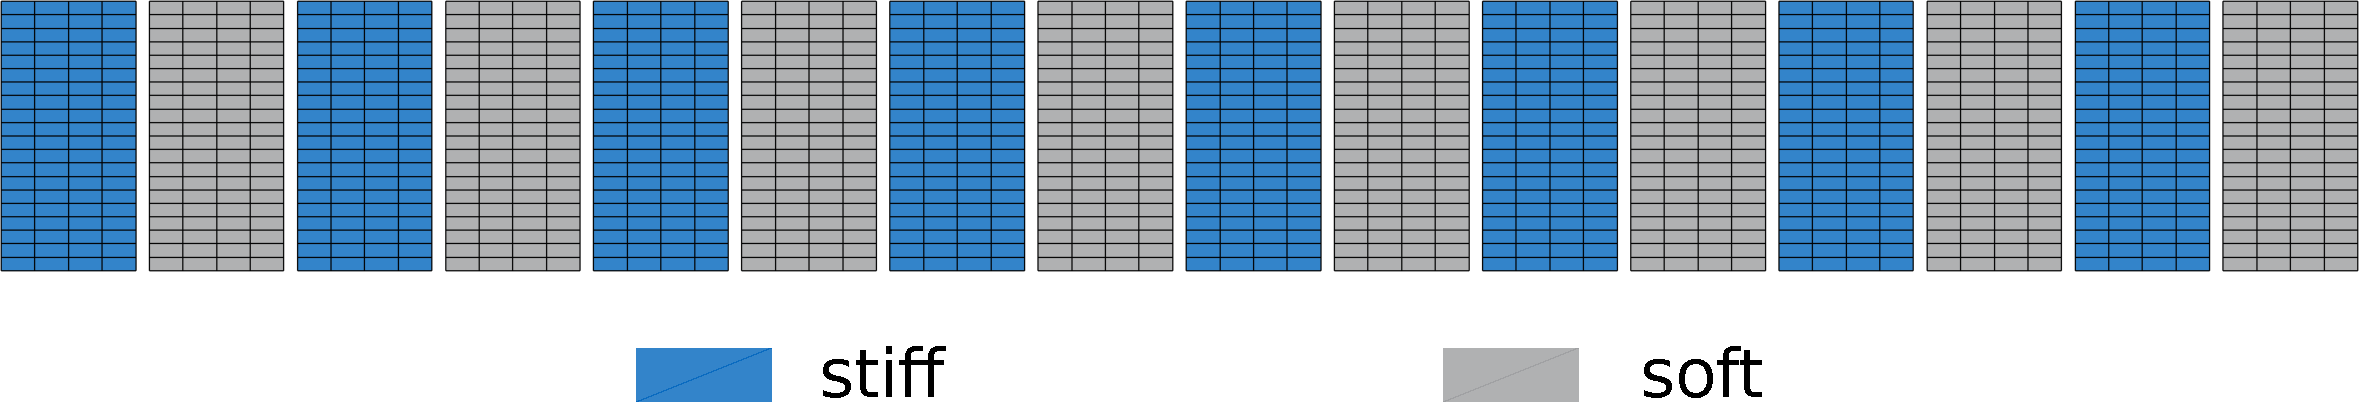
\includegraphics[width=0.6\textwidth]{\studypath/2016-08-22_HeterogenityType/setup/materials_vertical.pdf}
      \caption{Heterogeneities across the interface}
    \end{subfigure}
    \vskip\baselineskip
    \begin{subfigure}[b]{\textwidth}
      \centering
      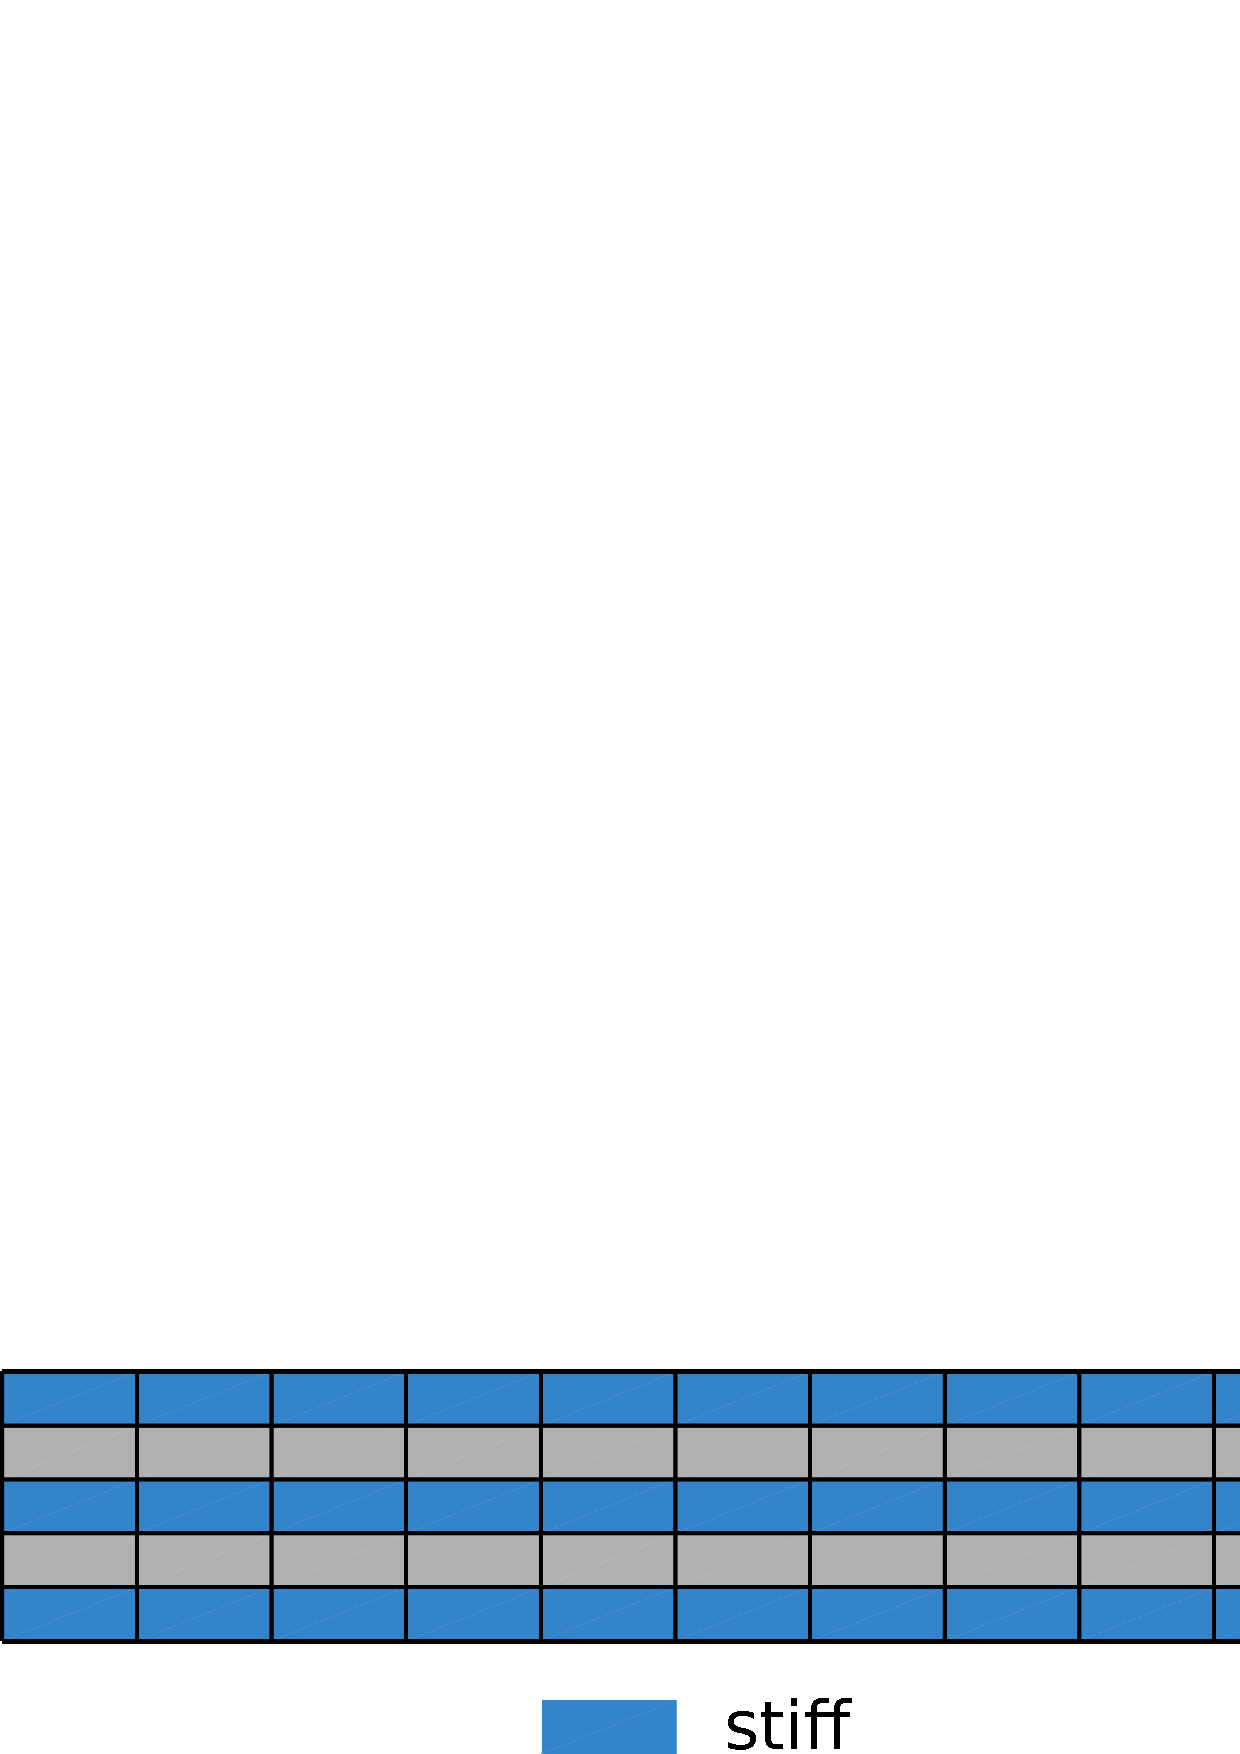
\includegraphics[width=0.6\textwidth]{\studypath/2016-08-22_HeterogenityType/setup/materials_horizontal.pdf}
      \caption{Heterogeneities along the interface}
    \end{subfigure}
    \vskip\baselineskip
    \begin{subfigure}[b]{\textwidth}
      \centering
      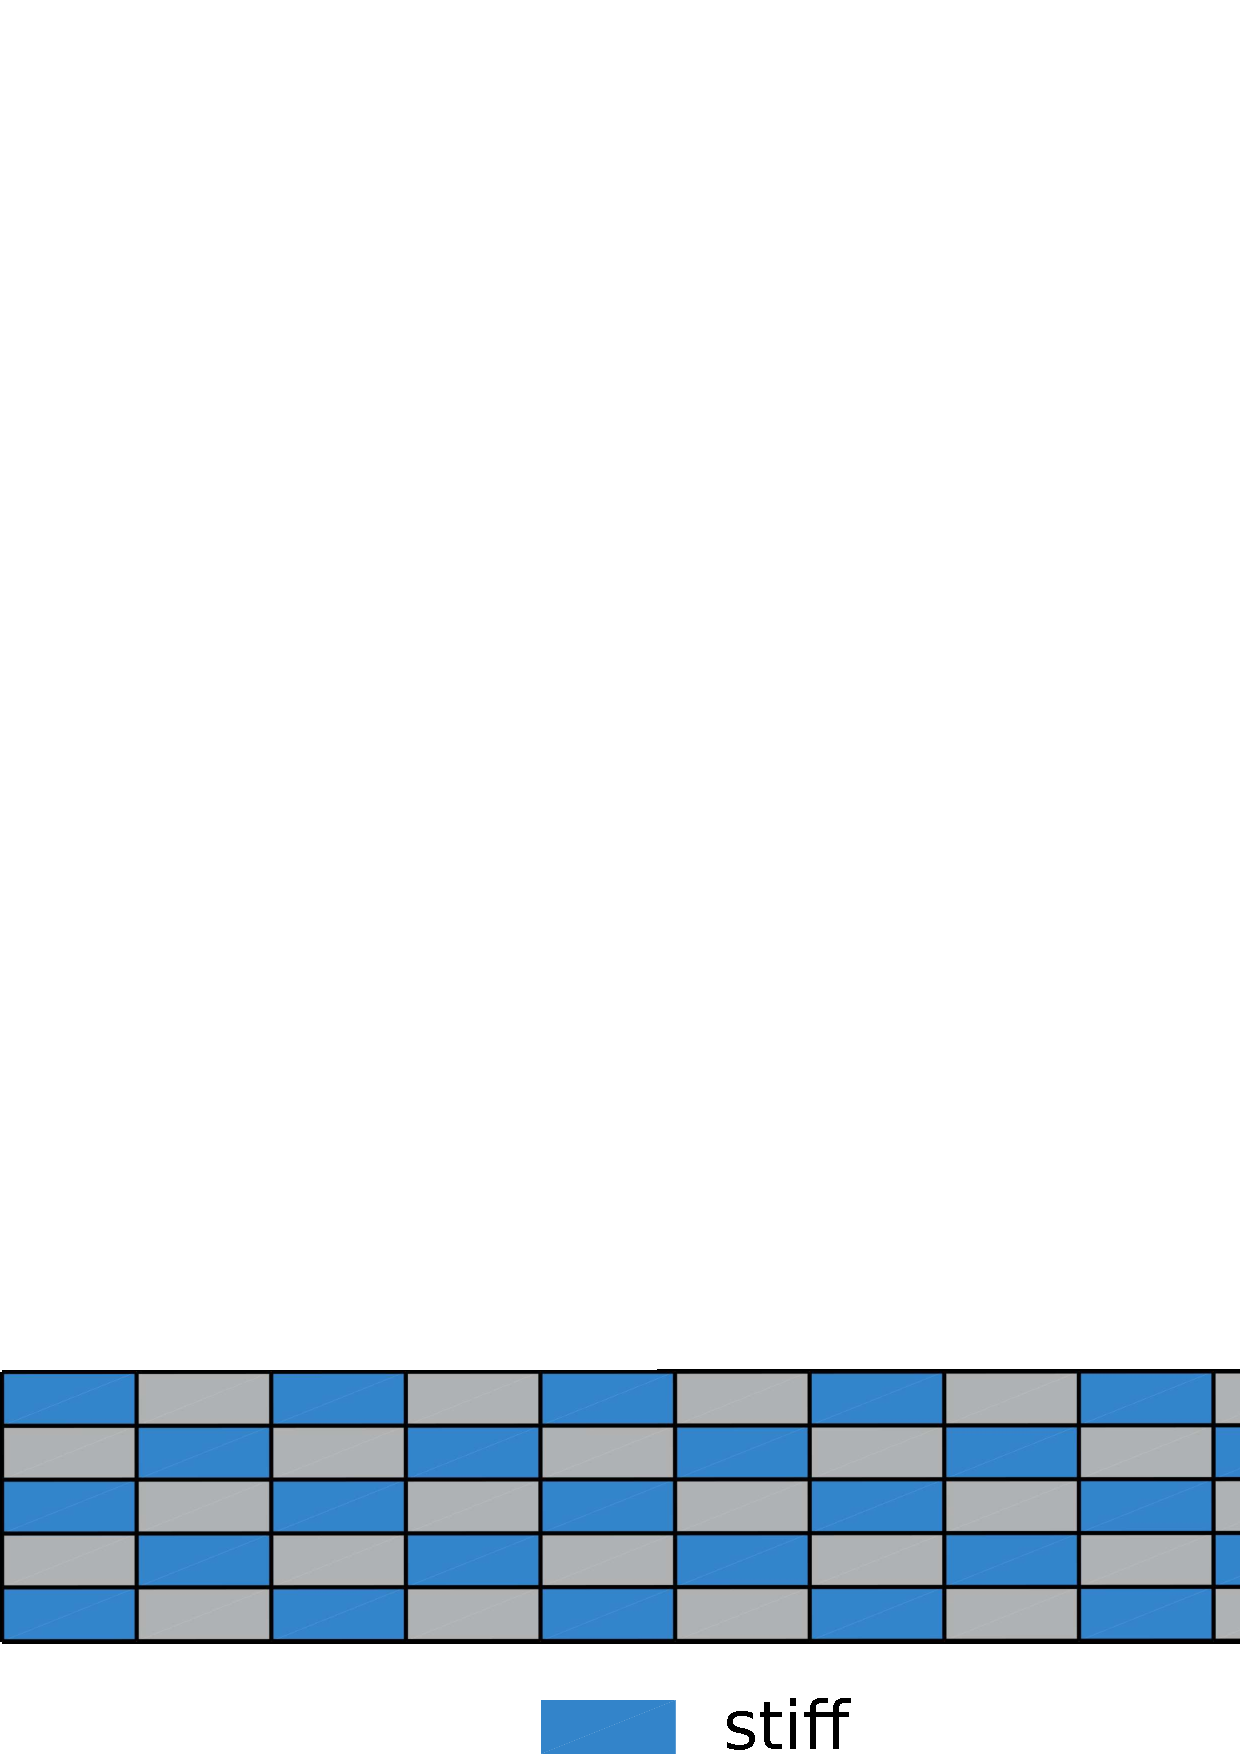
\includegraphics[width=0.6\textwidth]{\studypath/2016-08-22_HeterogenityType/setup/materials_checkerboard.pdf}
      \caption{Combined heterogeneities}
    \end{subfigure}
    \caption[Study of heterogeneities: material patterns]{Material patterns for the heterogeneity analysis. The substructuring has been done such, that the setup at the top shows heterogenities only across the interface and the middle one only along the interface. The checkerboard pattern at the bottom shows both, heterogeneities across and along the interface. The beams were clamped on the left side and subjected to a uniform downward force on the right.}
    \label{fig:heterogenity_materials_patterns}
  \end{center}
\end{figure}



\subsection{Heterogeneities across the interface}\label{sec:heterogeneities_across}
A typical example of heterogenities across the interface is described in the top of Figure~\ref{fig:heterogenity_materials_patterns}. The beam is clamped on the left face and subjected to a uniform downward force on the right face\\
The reason for the problems with this type of heterogeneity have been explained in Section~\ref{sec:precond}.\\
During the FETI iterations, intermediate solutions for the interface forces are found. Based on this force, a resulting displacement is predicted. In a standard, non scaled FETI-algorithm, this displacement is then applied in equal parts on the two substructure interfaces concerned. If now the substructure on one side of the interface is significantly stiffer, than the other one, this simple 50/50 approach, of course, leads to very wrong results. A possible solution to this problem is K-scaling, which has been derived in \cite{Farhat1995}. If not mentioned otherwise, this code does always use k-scaling and multiplicity scaling as explained in Section~\ref{sec:precond}.\\
The problem of heterogenities across the interface is visualized in Figure~\ref{fig:study_heterogeneity_results_across}.

\begin{figure}[tb]
  \begin{center}
    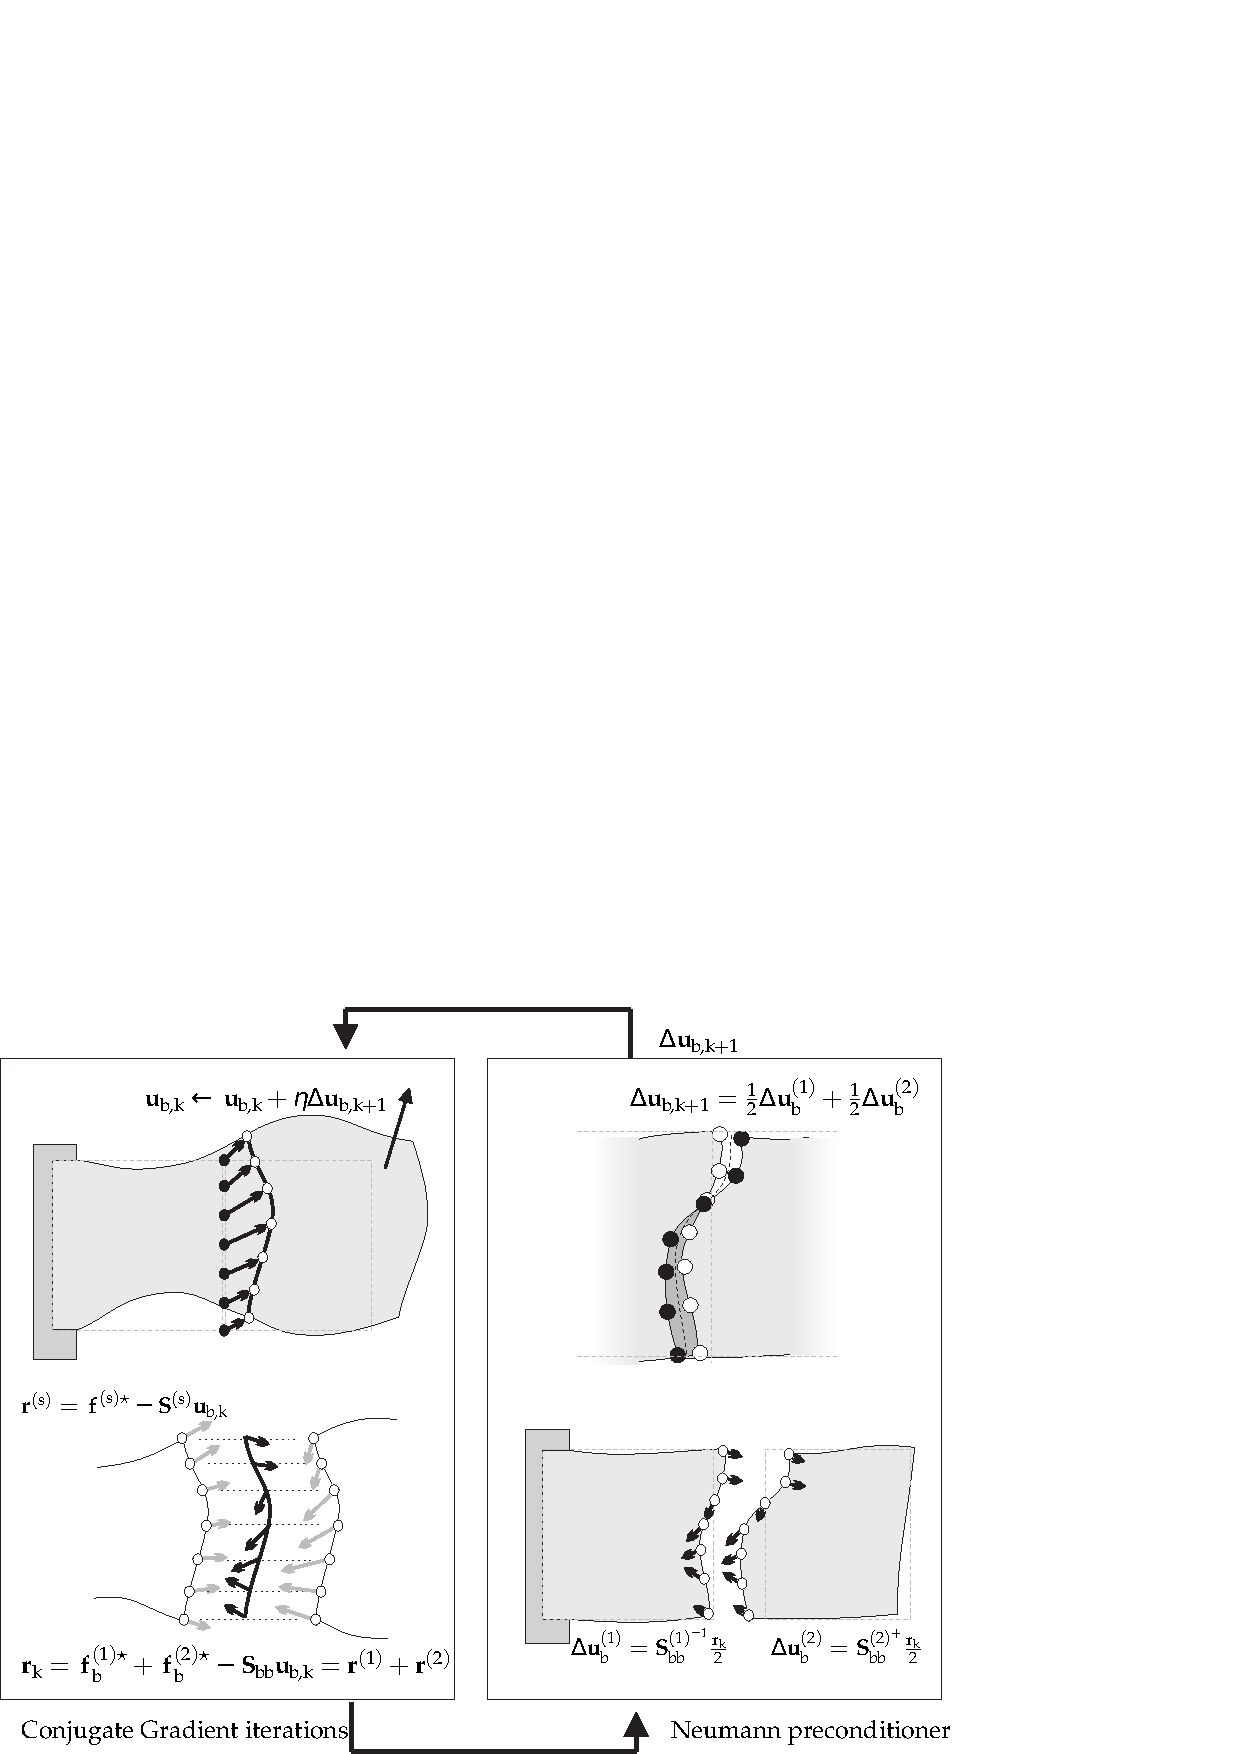
\includegraphics[width=0.5\textwidth]{./fig/pdf/problem_heterogenity.pdf}
    \caption[Study of heterogeneities across the interface: problem sketch]{Sketch of the Problem related to heterogenities across the interface. The figure was taken from~\cite{Rixen2013}. Through the simple sum of contributions in the preconditioner, all substructures contribute equally to the search direction. The Neumann step thus equally displaces both interface sides. If, however, one side of the interface shows a much higher stiffness than the other, the natural solution would actually be such, that the soft material shows a much higher displacement than the stiff one. If this discrepancy is not dealt with, convergence rates can be severely damaged. One possible solution would be K-scaling, as described in~\cite{Rixen1999a}. Also, thanks to its independent substructure-based search directions, FETI-S is not that susceptible to this problem.}
    \label{fig:problem_heterogenity_sketch}
  \end{center}
\end{figure}



\begin{figure}[tb]
  \begin{center}
    %\fbox{\subimport{./}{./fig/tikz/study_inclusion.tex}}
    \includestandalone{./fig/tikz/study_heterogenity_vstripes}
    \caption[Study of heterogeneities across the interface: \# iterations]{Results for the convergence analysis of the FETI algorithms for materials across the interface. The left figure shows the results without scaling, the left figure shows the results with scaling. The graphs do show two things. First of all, the multi preconditioned schemes seem to be far less effected by this type of heterogeneity, that the singe preconditioned ones.  Secondly, the scaling is very effective in reducing the iteration numbers for FETI-1. It also seems that K-scaling is mandatory for the FETI-2(Geneo) approach to work properly here. Since the numerical effort is low, it is therefore always recommended to use a k-scaling when high heterogeneities are present.}
    \label{fig:study_heterogeneity_results_across}
  \end{center}
\end{figure}

\begin{figure}
  \begin{center}
    \includestandalone{./fig/tikz/study_heterogenity_vstripes_residual}
    \caption[Study of heterogeneities across the interface: residua]{Residuum development for the convergence analysis of the FETI algorithms regarding heterogeneities across the interface, as described in the top of Figure~\ref{fig:heterogenity_materials_patterns}. Obviously K-scaling drastically improves performance here. The right figure shows that a PCG method(FETI-2) is capable of showing the same convergence rates as an MPCG one(FETI-S) provided that K-scaling is used. In that case, the reduced number of iterations of the FETI-S solver can be attributed to the reduced problem size solemnly. Finally, FETI-S seems to not have benefited much from the Scaling approach. This seems reasonable since substructures interfaces are optimized independently of one another anyway}
    \label{fig:heterogeneity_accross_residuum}
  \end{center}
\end{figure}

\begin{figure}
  \begin{center}
    \includestandalone{./fig/tikz/study_heterogenity_vstripes_adaptive}
    \caption[Study of heterogeneities across the interface: \# search directions]{Results for the convergence analysis of the FETI algorithms for materials across the interface, as depicted at the top of Figure~\ref{fig:heterogenity_materials_patterns}. This figure show the number of search directions used by the different adaptive schemes. Overall, FETI-AS shows superior results here. What is more, K-scaling seems to completely eliminate the problems of heterogeneities across the interface, since in that case, no difference can be observed between a stiffness ratio of 10 and a ratio of 1000.}
    \label{fig:heterogeneity_accross_numsdir}
  \end{center}
\end{figure}









\FloatBarrier
\subsection{Heterogeneities along the interface}\label{sec:heterogeneities_along}
Heterogeneities along the interface are somewhat more difficult. The ill-conditioning can not be coped with by simple scaling methods. The material distribution used for this analysis is provided in Figure~\ref{fig:heterogenity_materials_patterns}. Iteration numbers are provided in Figure~\ref{fig:study_heterogeneity_results_along}, residua development in Figure~\ref{fig:heterogeneity_along_residuum} and a visualization of the number of used search directions in Figure~\ref{fig:heterogeneity_along_numsdir}.
%%%\begin{figure}[tb]
%%%	\begin{center}
%%%	    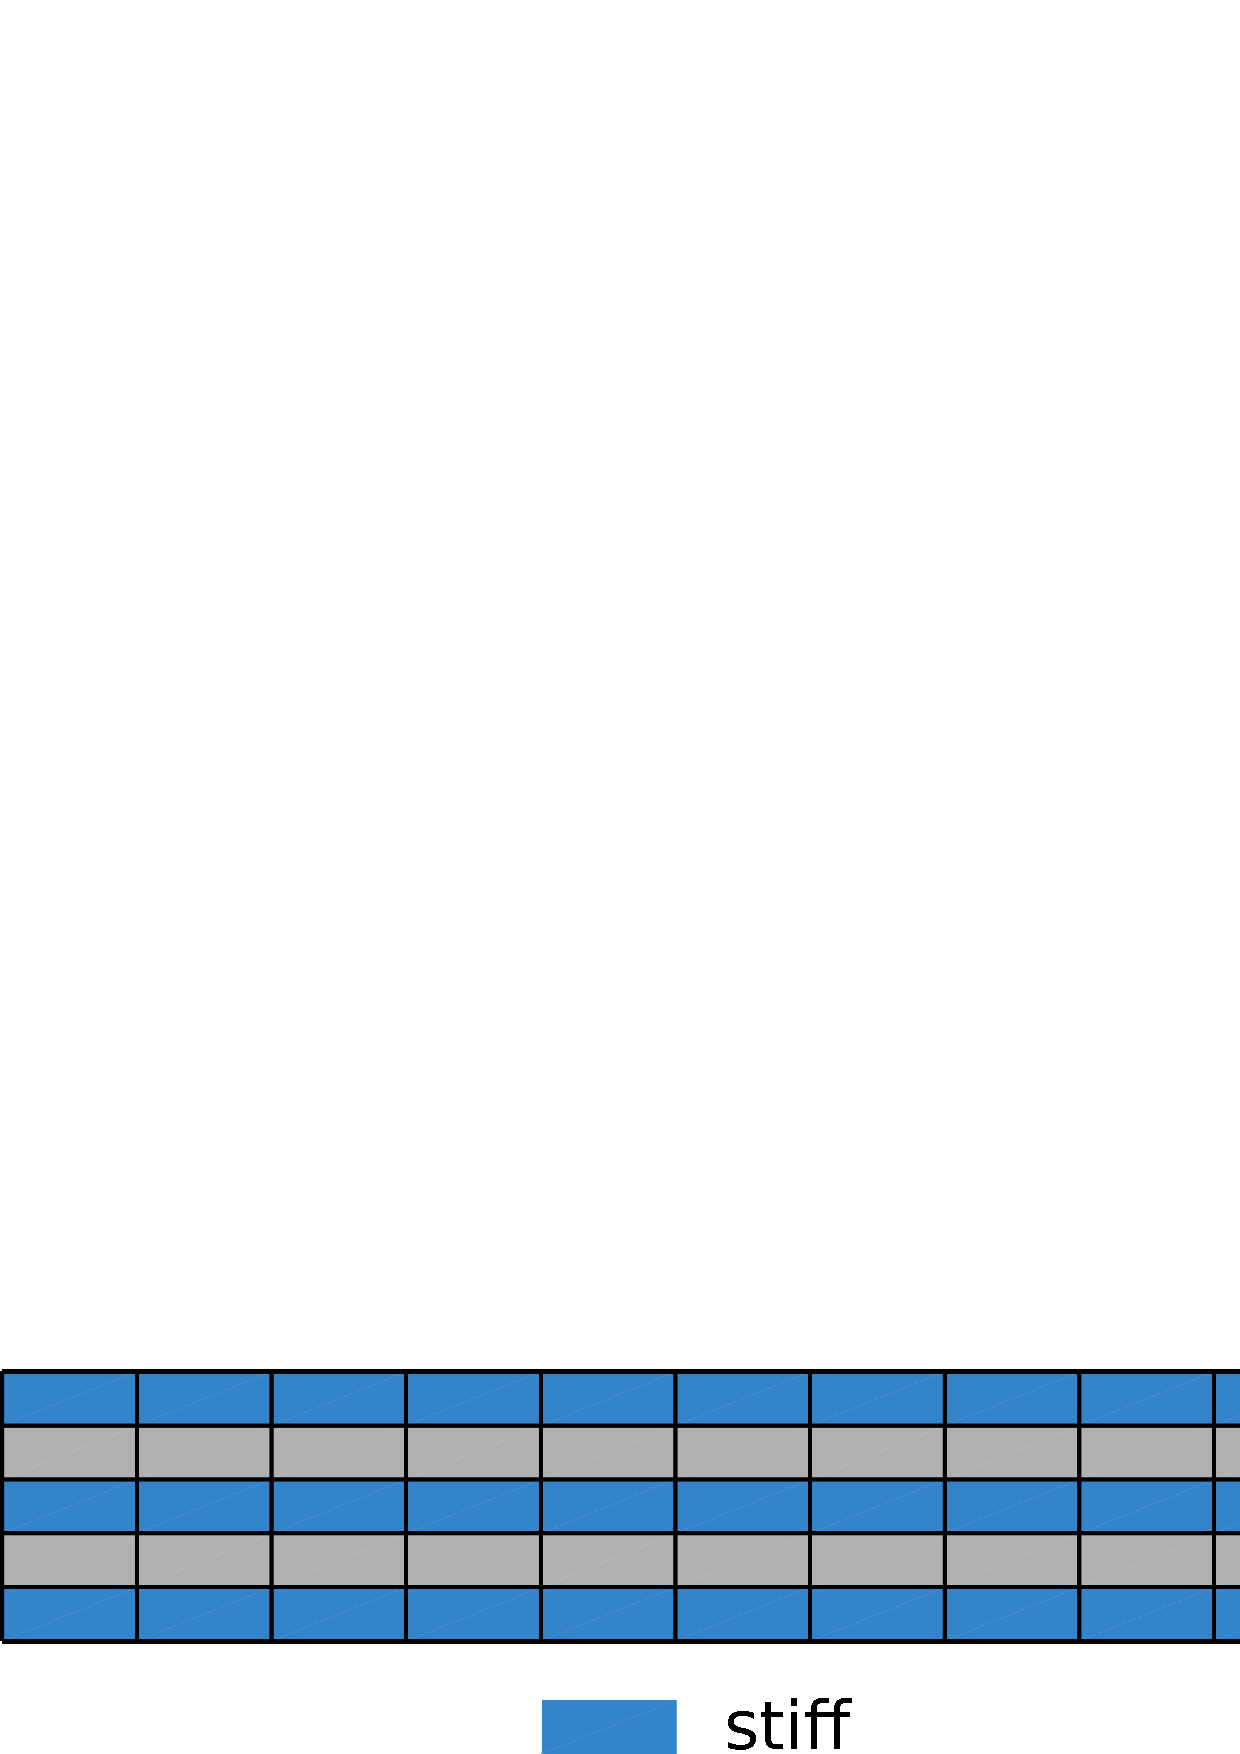
\includegraphics[width=0.5\textwidth]{\studypath/2016-08-22_HeterogenityType/setup/materials_horizontal.pdf}
%%%        \caption[Setup heterogeneity along interface]{Setup for the convergence analysis of the FETI algorithms with regards to heterogenities along the interface. The bearing of and the forces applied on the beam as well as its partitioning into substructures are visualized in Figure~\ref{fig:study_heterogenity_setup_bc}.}
%%%		\label{fig:study_heterogeneity_setup_along}
%%%    \end{center}
%%%\end{figure}

\begin{figure}[tb]
  \begin{center}
    %\fbox{\subimport{./}{./fig/tikz/study_inclusion.tex}}
    \includestandalone{./fig/tikz/study_heterogenity_hstripes}
    \caption[Study of heterogeneities along the interface: \# iterations]{Results for the convergence analysis of the FETI algorithms for materials along the interface. Again, FETI-2 shows severe problems. As expected, scaling does not improve the iteration counts significantly, since it is not designed to cope with this kind of heterogeneity. The multi preconditioned algorithms seem to be able to cope with the problem quite well. In contrast to the heterogeneities across the interface from Figure~\ref{fig:study_heterogeneity_results_across}, Geneo is capable of effectively detecting the bad modes and iteration counts can therefore be kept low successfully with FETI-2.}
    \label{fig:study_heterogeneity_results_along}
  \end{center}
\end{figure}

\begin{figure}
  \begin{center}
    \includestandalone{./fig/tikz/study_heterogenity_hstripes_residual}
    \caption[Study of heterogeneities along the interface: residua]{Residuum development for the convergence analysis of the FETI algorithms regarding heterogeneities along the interface, as described at the middle of Figure~\ref{fig:heterogenity_materials_patterns}. Obviously, K-scaling does not effect the convergence properties at all. What is more, MPCG methods show significantly better results than the PCG ones. In particular, Geneo performed much worse than for the case of heterogeneities across the interface. It remains to be analysed whether a larger coarse space would improve its properties, but, as explained earlier, increasing the coarse problem has significant drawbacks. }
    \label{fig:heterogeneity_along_residuum}
  \end{center}
\end{figure}

\begin{figure}
  \begin{center}
    \includestandalone{./fig/tikz/study_heterogenity_hstripes_adaptive}
    \caption[Study of heterogeneities across the interface: \# search directions]{Results for the convergence analysis of the FETI algorithms for materials along the interface, as described at the middle of Figure~\ref{fig:heterogenity_materials_patterns}. This figures visualizes the number of search directions used by the multi preconditioned schemes during the iterations. At least for the contraction factor of 0.999, the overall improvement is not satisfactory. FETI-AS, however still gives quite nice results with the standard parameters as defined in Section~\ref{sec:fetias}. }
    \label{fig:heterogeneity_along_numsdir}
  \end{center}
\end{figure}





\FloatBarrier
\subsection{Combined heterogeneities}\label{sec:heterogeneities_combined}
In real engineering problems, especially when automatic graph partitioners like Metis are used, one will most likely have to deal with a combined form of heterogeneity. Therefore a setup that contains both shall now be considered. The material pattern is depicted in the bottom of Figure~\ref{fig:heterogenity_materials_patterns}. Iteration numbers are provided in Figure~\ref{fig:study_heterogenity_combined}, numbers of used search directions in Figure~\ref{heterogeneity_combined_numsdir} and the residuum development in Figure~\ref{fig:heterogeneity_cboard_residuum}.


\begin{figure}[tb]
  \begin{center}
    %\fbox{\subimport{./}{./fig/tikz/study_inclusion.tex}}
    \includestandalone{./fig/tikz/study_heterogenity_cboard}
    \caption[Study of combined heterogeneities: \#iterations]{Results for the convergence analysis of the FETI algorithms for materials across and along the interface. As expected, FETI-1 performs very poorly. K-scaling does not really improved the iteration numbers, except for FETI-2, where we have already seen in Figure~\ref{fig:heterogeneity_along_numsdir} that it is not able to build an appropriate coarse grid for the case of heterogenities. As could be expected from Figures~\ref{fig:study_heterogeneity_results_across} and~\ref{fig:study_heterogeneity_results_along}, the multi-preconditioned algorithms show superior properties.}
    \label{fig:study_heterogenity_combined}
  \end{center}
\end{figure}

\begin{figure}
  \begin{center}
    \includestandalone{./fig/tikz/study_heterogenity_cboard_residual}
    \caption[Study of combined heterogeneities: residua]{Residuum development for the convergence analysis of the FETI algorithms regarding combined heterogeneities, as depicted at the bottom of Figure~\ref{fig:heterogenity_materials_patterns}. This figure shown the development of the residual over the iterations for al solvers. Obviously, K-scaling is not capable of significantly reducing the the total number of iterations, except for FETI-2(Geneo), where we have already observed that it seems to be necessary for the construction of an effective coarse space.}
    \label{fig:heterogeneity_cboard_residuum}
  \end{center}
\end{figure}

\begin{figure}
  \begin{center}
    \includestandalone{./fig/tikz/study_heterogenity_cboard_adaptive}
    \caption[Study of combined heterogeneities: \# search directions]{Results for the convergence analysis of the FETI algorithms regarding combined heterogeneities, as depicted at the middle of Figure~\ref{fig:heterogenity_materials_patterns}. This figure shows the number of search directions used by the multi preconditioned solvers for all iteration steps. Both FETI-AS ans FETI-FAS were capable of significantly reducing the total number of search directions used.}
    \label{heterogeneity_combined_numsdir}
  \end{center}
\end{figure}





\section{Partitioning}
For a domain decomposition method like FETI, the question of how to form the substructures comes naturally. Partitioning is typically done by automatic graph partitioning algorithms like Metis or Chaco. For some specific cases, however, it can be advantageous to choose partitions manually. Particularly, for the examples of a composite material, one can choose partitions such that the problems of heterogenities along the interface, as described in Section~\ref{sec:heterogeneities} are avoided.\\
Nonetheless, even automatic graph partitioners offer some parameters to choose from. This section is therefore denoted to an analysis of different partitioning approaches.
\\
Figure~\ref{fig:partitioning_schemes} shows the four different partitioning schemes considered. The plate is clamped on the left side and subjected to a uniform surface load in y-direction on the right face.
\\
The partitions have been chosen such, that the interface problem has roughly the same size on all four setups. We can note right at this point, that stripe-like partitioning like in the bottom two subfigures, is far less efficient when it comes to keeping the number of interface unknowns low. For an equally sized interface problem, the number of substructure is more than three times less than for the regular partitioning in the top-left figure, a potential weak-point when it comes to parallizability.\\
However, as~\cite{Farhat1991} writes, stripe-like partitioning may offer the advantage of a reduced interconnectivity in the substructure stiffness matrices, solving the local problems may becomes faster thus.
\\
The results of this analysis are presented in Figure~\ref{fig:study_partitioning_numiter}.



\begin{figure}[tbp]
  \centering
  \begin{subfigure}[b]{0.3\textwidth}
    \includegraphics[width=\textwidth]{/home/lukas/Desktop/SA_Thesis/studies/2016-08-10_Partitioning/setup/regular_6x6.png}
    \caption{regular partitioning}
  \end{subfigure}
  \hspace{1cm}
  \begin{subfigure}[b]{0.3\textwidth}
    \includegraphics[width=\textwidth]{/home/lukas/Desktop/SA_Thesis/studies/2016-08-10_Partitioning/setup/chaco_6x6.png}
    \caption{automatic partitioning}
  \end{subfigure}
  \vskip\baselineskip
  \begin{subfigure}[b]{0.3\textwidth}
    \includegraphics[width=\textwidth]{/home/lukas/Desktop/SA_Thesis/studies/2016-08-10_Partitioning/setup/chaco_11x1.png}
    \caption{vertical stripes}
  \end{subfigure}
  \hspace{1cm}
  \begin{subfigure}[b]{0.3\textwidth}
    \includegraphics[width=\textwidth]{/home/lukas/Desktop/SA_Thesis/studies/2016-08-10_Partitioning/setup/chaco_1x11.png}
    \caption{horizontal stripes}
  \end{subfigure}
  \caption[Study of partitioning schemes: setup]{Different partitioning schemes. The top left example was manually partitioned into equally sized substructures keeping the number of interface unknowns low. The top right example was partitioned using chaco in GMSH. Finally, the bottom two examples were created using the Simple Partitioner Plug-in of GMSH. Here, the number of subdomains had to be drastically reduced, in order to get roughly the same size for the interface problem as in the top two examples. No material heterogenities were considered here. The results of this analysis are presented in Figure~\ref{fig:study_partitioning_numiter}}
  \label{fig:partitioning_schemes}
\end{figure} 


\begin{figure}[tb]
  \begin{center}
    %\fbox{\subimport{./}{./fig/tikz/study_inclusion.tex}}
    \includestandalone{./fig/tikz/study_partitioning_numiter}
    \caption[Study of partitioning schemes: \# iterations]{Results for the analysis of different partitioning schemes as described in Figure~\ref{fig:partitioning_schemes}. Firstly, we note that no dramatic difference between the regular partitioning and the automatic partitioning can be observed. Secondly, the stripe-like partitions performed far worse than the first two ones. Although less susceptible than the others, even the multi preconditioned schemes showed an increase of close to 100\% in that case. Event though, it was not possible to collect actual CPU-times, due to the Matlab implementation, taking into account, that the total number of substructures had to be significantly reduced for the stripe-like setups, it can be safely assumed that the advantage of reduced interconnectivity in the local stiffness matrices for stripe-like partitions does not justify choosing such a partitioning scheme.\\
      A comparison with regards to the number of search directions between the multi preconditioned algorithms for this example is provided in Figure~\ref{fig:study_partitioning_numsdir}. }
    \label{fig:study_partitioning_numiter}
  \end{center}
\end{figure}


\begin{figure}
  \begin{center}
    %\fbox{\subimport{./}{./fig/tikz/study_inclusion.tex}}
    \includestandalone{./fig/tikz/study_partitioning_residual}
    \caption[Study of partitioning schemes: residua]{Residual development for the partitioning scheme analysis described in Figure~\ref{fig:partitioning_schemes}. One can note that FETI-2 with a Geneo coarse grid shows good convergence rate for the first two partitioning schemes, whereas the FETI-2 convergence rate is significantly lower for stripe-like partitioning schemes. It shall be noted, that in the first to schemes, 6 Geneo modes were used per substructure, whereas the last two ones were calculated with 18 Geneo modes per substructure, so that the overall size of the coarse problem is the same for all four examples.}
    \label{fig:study_partitioning_residual}
  \end{center}
\end{figure}

\begin{figure}[tb]
  \begin{center}
    %\fbox{\subimport{./}{./fig/tikz/study_inclusion.tex}}
    \includestandalone{./fig/tikz/study_partitioning_numsdir}
    \caption[Study of partitioning schemes: \# search directions]{Results for the analysis of different partitioning schemes as described in Figure~\ref{fig:partitioning_schemes}. Particularly, this figure shows the number of chosen search directions for FETI-S and FETI-FAS. Although probably not optimal, the FETI-FAS algorithm is quite efficient in reducing the total number of search directions during the iterations. All four examples have been calculated with the default FETI-FAS parameters, as described in Section~\ref{sec:fetifas}. }
    \label{fig:study_partitioning_numsdir}
  \end{center}
\end{figure}


\section{Incompressibility}
Another well known problem for convergence is material incompressibility. The problem has been thoroughly analysed in ~\cite{Vereecke2003}.
In a linear elasticity, plane strain formulation, one can write
\begin{align}
  \tensor{\sigma}=\tensor{D}\tensor{\epsilon} = 2 \mu \tensor{\epsilon}+\lambda (tr(\epsilon)) \dmat{1} = \frac{E}{1+\nu} \tensor{\epsilon} + \frac{\nu E}{(1+\nu)(1-2 \nu)} tr(\tensor{\epsilon}) \dmat{1} 
\end{align}

Obviously, this term becomes problematic if $\nu \rightarrow 0.5$. In fact, the condition number of the stiffness matrix increases both with $\nu$ and with the model size. The problem has been analysed for the introduced FETI type of solvers. The setup is described in Figure~\ref{fig:setup_problem_incompressibility}. No material heterogenities were used here, in order to focus on incompressibility exclusively.

\begin{figure}[tb]
  \begin{center}
    \includegraphics[width=0.45\textwidth]{\studypath/2016-08-19_Incompresibility/setup/setup.pdf}~\hspace{0.5cm}
    \includegraphics[width=0.36\textwidth]{\studypath/2016-08-19_Incompresibility/setup/partitioning.pdf}~
    \caption[Study of incompressibility handling: setup]{Setup for the incompressibility analysis. The beam is divided into 24 substructures as shown in the right subfigure. Both the bottom and the top surface are clamped. A constant pressure is applied on the left side. The results for different Poission numbers are shown in Figure~\ref{fig:results_problem_incompressibility}}
    \label{fig:setup_problem_incompressibility}
  \end{center}
\end{figure}



\begin{figure}[tb]
  \begin{center}
    %\fbox{\subimport{./}{./fig/tikz/study_inclusion.tex}}
    \includestandalone{./fig/tikz/study_incompressibility}
    \caption[Study of incompressibility handling: \# iterations]{Results for the incompressibility analysis described in Figure~\ref{fig:results_problem_incompressibility}. Since incompressibility is only a problem in plane-strain calculations the same calculations with a plane-stress formulations are provided in the right figure. The figures clearly show, that the standard FETI-1 solver is very vulnerable in nearly incompressible simulations.}
    \label{fig:results_problem_incompressibility}
  \end{center}
\end{figure}

\begin{figure}%[tb]
  \begin{center}
    %\fbox{\subimport{./}{./fig/tikz/study_inclusion.tex}}
    \includestandalone{./fig/tikz/study_incompressibility_adaptive}
    \caption[Study of incompressibility handling: \# search directions]{Results for the incompressibility analysis described in Figure~\ref{fig:results_problem_incompressibility}. This figure shows the number of search directions used by the multi preconditioned schemes during the iterations. FETI-AS is not able to reduce search at all with the standard parameters here. FETI-AS does, but it tends to overshoot when approaching $\nu\rightarrow 0.5$. Overall, incompressibility seem to be a problem, where the adaptive schemes show no advantage compared to FETI-S}
    \label{fig:todo}
  \end{center}
\end{figure}

\FloatBarrier
\section{Inclusion}
The previous sections have indicated that parameter jumps along or across the interface pose a serious problem for DD-type of solvers.\\
One can however also create homogeneous interface examples, that still lead to highly increased iteration numbers. From an engineering point of view, this is due to substructures that show fundamentally different stiffness properties when considered separately than when considered in composite with the other substructures. The following considerations are inspired by~\cite{Gosselet2015}. The setup is briefly described in Figure~\ref{fig:setup_inclusion_problem} and the numerical results are presented in Figure~\ref{fig:results_inclusion_problem}.\\
The number of search directions used my the multi preconditioned solver is depicted in Figure~\ref{fig:results_inclusion_problem_adaptive}. Moreover, an visualization of the development of the residuum is provided in Figure~\ref{fig:results_inclusion_problem_residuum}.

\begin{figure}[tb]
  \begin{center}
    \includegraphics[width=0.4\textwidth]{\studypath/2016-08-19_Inclusion/setup/setup.pdf}~
    \hspace{1cm}~
    \includegraphics[width=0.35\textwidth]{\studypath/2016-08-19_Inclusion/setup/partitioning.pdf}
    \caption[Study of inclusion handling: setup]{Setup for the inclusion analysis. The left figure shows the material distribution. The right figure depicts the partitioning into substructures. As shown, every substructure consists of a lattice around the substructure border and another material within (inclusion). An setup like this as coefficient jumps neighter along nor across the interface. Nevertheless FETI-solver are challenged by it. Figure~\ref{fig:results_inclusion_problem} shows the iteration counts for the different FETI-algorithms}
    \label{fig:setup_inclusion_problem}
  \end{center}
\end{figure}	

\begin{figure}[tb]
  \begin{center}
    %\fbox{\subimport{./}{./fig/tikz/study_inclusion.tex}}
    \includestandalone{./fig/tikz/study_inclusion}
    \caption[Study of inclusion handling: \# iterations]{Results for the inclusion problems as described in Figure~\ref{fig:setup_inclusion_problem}. The top two figures show the calculations with the default lumped preconditioner, the bottom ones with a full Dirichlet preconditioner(see Section~\ref{sec:precond}. The left figures were calculated with inclusion to substructure ration of $\frac{L_{inclusion}}{L_{substructure}}=0.9$, the right figures with $\frac{L_{inclusion}}{L_{substructure}}=0.95$.  The graphs show that FETI-S and FETI-2(Geneo) show less sever increases in the iteration numbers than FETI-1, when the stiffness ratio $\frac{E_{inclusion}}{E_{lattice}}$ is decreased. As expected, the problematic case is the one with soft inclusions inside a stiff lattice. In that case, the solver drastically underestimates the deformation. The overestimation of deformation for the contrary case is not critical. What is more, one can also notice that FETI-2 is obviously not able to correctly detect the bad modes, when a lumped preconditioner is used. This is intuitive when looking at the very definition of the two preconditioner types in Equations~\eqref{eq:precond}\eqref{eq:precond_mscaled}\eqref{eq:precond_kscaled}. Since the lumped preconditioner neglects the Inner stiffness components $\stiffmat_{ii}$, no information abut the inner stiffness change enters the Geneo algorithms.}
    \label{fig:results_inclusion_problem}
  \end{center}
\end{figure}

\begin{figure}[tb]
  \begin{center}
    \subimport{./}{./fig/tikz/study_inclusion_residual}
    \caption[Study of inclusion handling: residua]{Residuum development for the inclusion analysis with lumped and Dirichlet preconditioners and soft as well as stiff inclusions. The case of hard inclusions obviously does not pose any problems. As mentioned in Figure~\ref{fig:results_inclusion_problem} the top two figures again confirm, that Geneo can only play out its advantages in terms of convergence rate, when the Dirichlet preconditioner is used. Otherwise it is not able to detect soft inclusions. However, the Dirichlet preconditioner comes with a significantly increased price, as outlined in Section~\ref{sec:precond}. }
    \label{fig:results_inclusion_problem_residuum}
  \end{center}
\end{figure}


\begin{figure}[tb]
  \begin{center}
    \subimport{./}{./fig/tikz/study_inclusion_adaptive}
    %\includestandalone{./fig/tikz/study_inclusion_adaptive}
    \caption[Study of inclusion handling: \# search directions with lumped preconditioner]{Results for the inclusion problems as described in Figure~\ref{fig:setup_inclusion_problem} with a lumped preconditioner. This plots compare the number of search directions used during the iterations of the FETI-S and the FETI-FAS algorithm. For the top two figures, the FETI-FAS algorithms shows mediocre results.For the bottom figure, FETI-FAS successfully detects the expandability of almost all search directions ans thereby reduced the computational effort significantly. The application of FETI-FAS did not pose any problems here, since the standard parameters as introduces in Section~\ref{sec:default_parameters} were used. }
    \label{fig:results_inclusion_problem_adaptive}
  \end{center}
\end{figure}

\begin{figure}[tb]
  \begin{center}
    \subimport{./}{./fig/tikz/study_inclusion_adaptive_dirich}
    %\includestandalone{./fig/tikz/study_inclusion_adaptive}
    \caption[Study of inclusion handling: \# search directions with Dirichlet preconditioner]{Results for the inclusion problems as described in Figure~\ref{fig:setup_inclusion_problem} wit a Dirichlet Preconditioner. This plots compare the number of search directions used during the iterations of the FETI-S and the FETI-FAS algorithm. When compared to Figure~\ref{fig:results_inclusion_problem_adaptive}, we note that the appropriate choice of the contraction factor $\tau$ is obviously, among others, dependent on the preconditioner type used, while FETI-FAS  performs reasonably well for both cases.}
    \label{fig:results_inclusion_problem_adaptive_dirich}
  \end{center}
\end{figure}


